\documentclass[10pt]{article}

\usepackage{multirow}
\usepackage{rotating,graphicx}
%\usepackage{wrapfig}
\usepackage{amssymb}
\usepackage{amsmath}
\usepackage{lscape}
\usepackage{times}
\usepackage{color}  % For \textcolor and \color % Ex. : \textcolor{red}{Text colored with} ; {\color{red}Text colored with}
\usepackage{soul}   % For \hl{ highlighted text} ; \sethlcolor{colorname}
%\usepackage[table]{xcolor}
\usepackage{xcolor,colortbl}
\usepackage{capt-of}
\usepackage{textcomp}  % allows \textonehalf,  \textonequarter, or else
%\usepackage{mathcomp}  % make it math compatible

\oddsidemargin =-0.6in
\evensidemargin=-0.6in
%\textwidth=7.6in   % owl
 \textwidth=7.8in % laptop
\textheight=10.2in
% \topmargin=-.25in   % owl
 \topmargin=-1.in    % laptop
\footskip=-.0in

\newcommand{\Bl}{\ensuremath{B_{{low}}}}
\newcommand{\Bh}{\ensuremath{B_{{high}}}}
\newcommand{\Il}{\ensuremath{I_{{low}}}}
\newcommand{\Ih}{\ensuremath{I_{{high}}}}
\newcommand{\Br}{\ensuremath{B\! \rho}}
\newcommand{\CE}{concentration ellipse}
\newcommand{\CES}{CE-$\rm \mathcal{S}$}
\newcommand{\dEE}{\small \ensuremath{\frac{dE}{E}}}
\newcommand{\eg}{\ensuremath{\it e.g.}}
\newcommand{\Ha}{\ensuremath{\mathcal{H}}}
\newcommand{\Sa}{\ensuremath{\mathcal{S}}}
\newcommand{\vs}{\ensuremath{\it vs.}}
\newcommand{\ie}{\ensuremath{\it i.e.}}
\newcommand{\hbrk}{\hfill \break}
\newcommand{\sr}{synchrotron radiation}
\newcommand{\SRl}{SR loss}
\newcommand{\x}{\ensuremath{x}} 
\newcommand{\xp}{\ensuremath{{x'}}}
\newcommand{\z}{\ensuremath{z} }
\newcommand{\zp}{\ensuremath{{z'}}}
\newcommand{\y}{\ensuremath{y} }
\newcommand{\yp}{\ensuremath{{y'}}}
\newcommand{\dl}{\ensuremath{{\delta l}}} 
\newcommand{\dE}{\ensuremath{{\delta E}}}
\newcommand{\X}{\ensuremath{X} }
\newcommand{\Xp}{\ensuremath{{X'}}}
\newcommand{\Z}{\ensuremath{Z} }
\newcommand{\zg}{Zgoubi}
\newcommand{\Zp}{\ensuremath{{Z'}}}
\newcommand{\Y}{\ensuremath{Y} }
\newcommand{\Yp}{\ensuremath{{Y'}}}
\newcommand{\Len}{\ensuremath{l} }
\newcommand{\Mom}{\ensuremath{E}}
\newcommand{\Sx}{\ensuremath{\mathcal{S}_x}}
\newcommand{\Sy}{\ensuremath{\mathcal{S}_y}}
\newcommand{\Sz}{\ensuremath{\mathcal{S}_z}}

\newcommand{\C}{\ensuremath{\mathcal{C}}}
\newcommand{\D}{\ensuremath{\mathcal{D}}}
\newcommand{\HH}{\ensuremath{\mathcal{H}}}
\newcommand{\bHH}{\bar \HH}
\newcommand{\com}{{center of mass}}
\newcommand{\lab}{{laboratory frame}}
\newcommand{\LL}{\ensuremath{\mathcal{L}}}
\newcommand{\rms}{\ensuremath{rms}}
\newcommand{\wrt}{{with respect to}}

\newcommand{\bull}{\ensuremath{\bullet~}}
\newcommand{\cf}{\ensuremath{\textsl{cf.}}}
\newcommand{\bhel}{\ensuremath{\mathbf{^3He^{2+}}}}
\newcommand{\hel}{\ensuremath{\mathrm{^3He^{2+}}}}
\newcommand{\nib}{\noindent \ensuremath{\bullet~}}
\newcommand{\snib}{\noindent {\small \ensuremath{\bullet~}}}
\newcommand{\nid}{\noindent \ensuremath{\diamond~}}
\newcommand{\snid}{\noindent {\small \ensuremath{\diamond~}}}
\newcommand{\nin}{\noindent~}
\newcommand{\no}{\ensuremath{\mathbf{\vec n_0}}}
\newcommand{\MC}{Monte~Carlo}
\newcommand{\p}{\ensuremath{\mathbf{p}}}
\newcommand{\pp}{$\rm p\! \! \uparrow$}

\definecolor{orange}{rgb}{1,0.5,0}
\definecolor{yelloworange}{rgb}{1,.647,0}
\newcommand{\black}{\color{black}}
\newcommand{\red}{\color{red}}
\newcommand{\green}{\color{green}}
\newcommand{\blue}{\color{blue}}
\newcommand{\yo}{\color{yelloworange}}

\newcommand{\referenceA}{\rm  }
\newcommand{\referenceB}{\rm }
\newcommand{\referenceC}{\rm }

\pagestyle{headings}
\markboth{\small  \referenceA ~ ~   \referenceB ~ ~  \referenceC \hfill }
         {\small  \referenceA ~ ~   \referenceB ~ ~  \referenceC \hfill }


\begin{document}

\thispagestyle{empty}

\begin{minipage}{1.\linewidth}
\bf
  \flushright{F. M\'eot}
\vspace{-2ex}
  
  \flushright{BNL C-AD}
\vspace{-2ex}
  
  \flushright{Zgoubi 2019 Workshop, Boulder, CO}
\vspace{-2ex}
  
\flushright{24-29 Aug. 2019} 
\end{minipage}


\vspace{5ex}

\centerline{\LARGE \bf
  An Introduction to the Wien Filter  
}

~

\centerline{\LARGE \bf
 A Parallel Plate Electrostatic Deflector
}

\vspace{5ex}
\author{
F.~M\'eot
\\
Collider-Accelerator Department, BNL, Upton, NY 11973 \\
}



\texttt{WIENFILTER} is used in this exercise (pp.~168 and 306 in the Users' Guide), with B=0  so that the Wien filter operates as a simple parallel plate electrostatic deflector.

Note: \texttt{ELMIR, ELMIRC} and even \texttt{ELMULT} or \texttt{EBMULT}  could be used as well, they would be able to provide this dipole $ \vec E$ field simulations (see "Optical elements versus keywords'' in the Users' Guide).


\section*{Working hypotheses}

\nib The Wien filter length is $ L$. Take $ \vec E =\vec E_Y \parallel \vec Y$.
Take  hard-edge E-field model  so to allow tight comparison with theory~\footnote{G.\,Leleux, INSTN Saclay, 1978 (unpublished)}.

\begin{minipage}{.69\linewidth}
\nib In order to check numerical outcomes: the expected trajectory is a catenary:
%
$$ Y_{th}(X) = \frac{E_i}{qE_Y} \left( \cosh \dfrac{qE_Y X}{\beta_i E_i } -1 \right)$$
with $E_i$  initial total energy, $c\beta_i$ initial velocity, $q$  particle charge

~

\nib Spin rotation: assume we manage to maintain $\vec E \perp \vec v$, namely, $\vec v = v_X$, always. Thus expected spin rotation over L  is (Eq.\,2.1.4 in Zgoubi Users' Guide)
$$ \theta_s = (a\gamma+\dfrac{\gamma}{1+a\gamma})\beta_X^2 \dfrac{E_YcL}{B\rho}  $$

\end{minipage} \hfill
\begin{minipage}{.3\linewidth}
  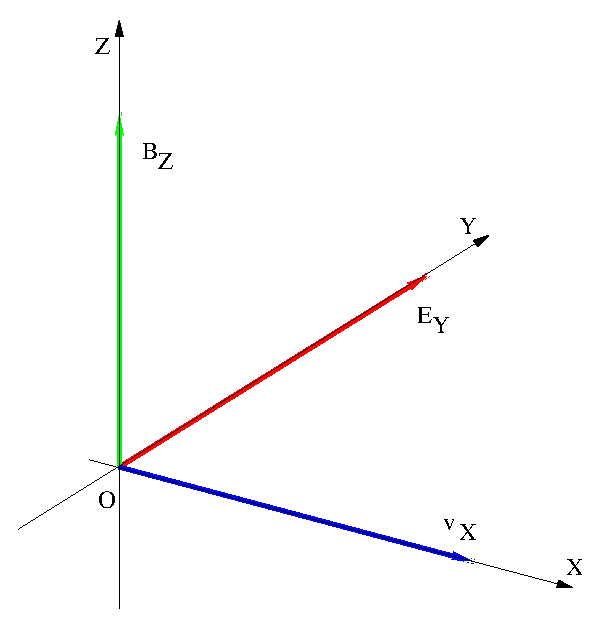
\includegraphics[width=0.99\linewidth]{wienF.eps}
\end{minipage}


\section*{ Numerical experience }

\nin 1/ Let's  walk through the fortran, see what happens when the execution pointer meets 'WIENFILTER'  in zgoubi.dat sequence...

Open zgoubi.f $\Rightarrow$ look for WIENFILTER. Look into include/LSTKEY.H  $\Rightarrow$  look for 'CALL RWIENF', look into rwienf.f
$\Rightarrow$  look for 'CALL QUASEX', look into quasex.f $\Rightarrow$ look for 'CALL CHXC', look into chxc.f,
look for WIENFILT therein
$\Rightarrow$ look for 'CALL TRANSF' in quasex, look into transf.f $\Rightarrow$ look into integr.f: it pushes the particles, one by one,
through the Wien filter (and any other element) $\Rightarrow$  look for 'CALL CHAMC', 'CALL CHAMK', 'CALL DEVTRA'.

~

\nin 2/ Set up a Wien filter in zgoubi with $ E_Y=0.98$\,MV/m,  $ L=0.5$\,m.
Consider an electron with 350\,keV energy. 

 Run zgoubi and check (in zgoubi.res)  final $Y(X\equiv L)$,  particle deviation, compare with result from catenary equation above.

~

\nin 3/ Check the effect of step size:

Using REBELOTE, get a scan of Y values for $ \Delta s = .001:10$\,cm.
   Plot $(Y-Y_{th})/Y_{th}$ versus step size (can use gnuplot to plot data read from zgoubi.fai).

   ~

   \nin 4/
   Force Y=0 across the Wien filter, by means of OPTION/CONSTY.

   Check the rotation of an initial $\vec S \equiv \vec S_X$, at the downstream end of the condenser (X=L), compare to expected $\theta_s$. 

Check convergence of result versus integration step size. 
   
   ~

   \nin 5/ Add fringe-fields.

   3.a  Plot the particle trajectory and the $E_Y$ and $B_Z$ fields along the trajectory.

   3.b  Plot particle energy versus distance, conclude on the importance of fringe fields as to 6-D symplecticity. 

   ~




   \clearpage

   \section*{Answers}

   1/
   
   \nib A xcell sheet can be used...

   Expected $Y(X=L)= \dfrac{511+350}{-980} \left( \cosh\dfrac{-980 \times 0.5}{\sqrt{((511+350)^2-511^2}} -1\right)= -22.8948628$ \ \ \ ($E_Y>0$ and $q<0$    so $Y_{final} <0$.

   \nib Expected spin rottion is $ \theta_s \approx (1.68\times1.16\, 10^{-3} +\dfrac{1.68}{2.68})\times 0.8^2 \dfrac{0.8\times 3\,10^8\times 0.5}{2.31\, 10^{-3}} *** \approx 20.526$

   \bigskip

\nib   Input data file (it can be copy-pasted, as is, and run):

{\tiny
\begin{verbatim}
E field only
 'OBJET'                                                                                                      1
2.3114795386518345           ! Rigidity of a 350 keV electron.
2
3  1                         ! 3 electrons, reason: see SPNTRK below.
0.  0. 0. 0. 0. 1. 'o'
0.  0. 0. 0. 0. 1. 'o'
0.  0. 0. 0. 0. 1. 'o'
1 1 1
 
 'PARTICUL'                                                                                                   2
ELECTRON
 'SPNTRK'                      ! Allows chceking rotation of all 3 spin components.                           3
4                             ! (they are computed independently by zgoubi)
1. 0. 0.
0. 1. 0.
0. 0. 1.
 
 'WIENFILT'                                                                                                   4
2                             ! Log to zgoubi.plt, every other 10 step.
0.5  0.98e6 0.    1
0. 0. 0.     ! 20. 5. 5.      ! Hard-edge entrance face.
0.2401  1.8639  -0.5572  0.3904 0. 0.
0.2401  1.8639  -0.5572  0.3904 0. 0.
0. 0. 0.     ! 20. 5. 5.      ! Hard-edge exit face.
0.2401  1.8639  -0.5572  0.3904 0. 0.
0.2401  1.8639  -0.5572  0.3904 0. 0.
.1
1. 0. 0. 0.
 'FAISCEAU'     ! Get some trajectory and some                                                                5
 
 'SPNPRT'  MATRIX                                                                                             6
 
 'SYSTEM'                                                                                                     7
1
gnuplot <./gnuplot_trajectory.gnu &
 'END'                                                                                                        8
\end{verbatim}
}

\bigskip

\nib Excerpts, from zgoubi.res:


- Particle and kinematics data:

{\tiny
\begin{verbatim}
*******************************************************************************************************************************
      2  Keyword, label(s) :  PARTICUL                                                                                 IPASS= 1

     Particle  properties :
     ELECTRON
                     Mass          =   0.510999        MeV/c2
                     Charge        =  -1.602176E-19    C     
                     G  factor     =   1.159652E-03          
                     COM life-time =   1.000000E+99    s     

              Reference  data :
                    mag. rigidity (kG.cm)   :   2.3114795      =p/q, such that dev.=B*L/rigidity
                    mass (MeV/c2)           :  0.51099895    
                    momentum (MeV/c)        : -0.69296413    
                    energy, total (MeV)     :  0.86099896    
                    energy, kinetic (MeV)   :  0.35000002    
                    beta = v/c              : -0.8048373615    
                    gamma                   :   1.684932950    
                    beta*gamma              :  -1.356096989    
                    G*gamma                 :  1.9539361699E-03
                    electric rigidity (MeV) : -0.5577234240    =T[eV]*(gamma+1)/gamma, such that dev.=E*L/rigidity
*******************************************************************************************************************************
\end{verbatim}
}

- final coordinates:

{\tiny
\begin{verbatim}
*******************************************************************************************************************************
      5  Keyword, label(s) :  FAISCEAU                                                                                 IPASS= 1

0                                             TRACE DU FAISCEAU
                                           (follows element #      4)
                                                  3 TRAJECTOIRES

                                   OBJET                                                  FAISCEAU

          D       Y(cm)     T(mr)     Z(cm)     P(mr)       S(cm)      D-1     Y(cm)    T(mr)    Z(cm)    P(mr)      S(cm)

o  1   1.0000     0.000     0.000     0.000     0.000      0.0000    0.3817  -22.893 -761.600    0.000    0.000   5.637547E+01     1
               Time of flight (mus) :  2.24897868E-03 mass (MeV/c2) :  0.510999    
o  1   1.0000     0.000     0.000     0.000     0.000      0.0000    0.3817  -22.893 -761.600    0.000    0.000   5.637547E+01     2
               Time of flight (mus) :  2.24897868E-03 mass (MeV/c2) :  0.510999    
o  1   1.0000     0.000     0.000     0.000     0.000      0.0000    0.3817  -22.893 -761.600    0.000    0.000   5.637547E+01     3
               Time of flight (mus) :  2.24897868E-03 mass (MeV/c2) :  0.510999    
*******************************************************************************************************************************
\end{verbatim}
}


\clearpage

2/


\nib   Input data file (it can be copy-pasted, as is, and run):

REBELOTE does the scan. Its option ``1'' ensures the change, parameter ``80''  in WIENFILT, takes NPASS = 60 different values
in [0.01,10.].

{\tiny
\begin{verbatim}
E field only
 'OBJET'                                                                                                      1
2.3114795386518345           ! Rigidity of a 350 keV electron.
2
3  1                         ! 3 electrons, reason: see SPNTRK below.
0.  0. 0. 0. 0. 1. 'o'
0.  0. 0. 0. 0. 1. 'o'
0.  0. 0. 0. 0. 1. 'o'
1 1 1
 
 'PARTICUL'                                                                                                   2
ELECTRON
 
 'WIENFILT'                                                                                                   3
0                             ! Log to zgoubi.plt, every other 10 step.
0.5  0.98e6 0.    1
0. 0. 0.     ! 20. 5. 5.      ! Hard-edge entrance face.
0.2401  1.8639  -0.5572  0.3904 0. 0.
0.2401  1.8639  -0.5572  0.3904 0. 0.
0. 0. 0.     ! 20. 5. 5.      ! Hard-edge exit face.
0.2401  1.8639  -0.5572  0.3904 0. 0.
0.2401  1.8639  -0.5572  0.3904 0. 0.
.1
1. 0. 0. 0.
 
 'FAISCEAU'    ! Get some trajectory data
 'DRIFT'       ! This gives more digits on coordinates (printing to zgoubi.fai would, as well)                5
0.
 'FAISTORE'    ! For use by gnuplot.                                                                          6
zgoubi.fai
1
 
 'REBELOTE'                                                                                                   7
2000  1.1  0 1
1
WIENFILT 80 0.001:10.      ! Step size is parameter #80 in WIENFILT
 
 'SYSTEM'                                                                                                     8
1
gnuplot <././gnuplot_scanStepSize.gnu &
 
 'END'                                                                                                        9
\end{verbatim}
}

\bigskip

A convenient gnuplot file to plot the step size scan:
{\tiny
\begin{verbatim}
set xlabel "step size [cm]"
set x2label "step size (zoomed) [cm]"
set ylabel "|Y-Y_{expected}|/Y_{expected} "
set y2label "|Y-Y_{expected}|/Y_{expected} (zoomed)"

set k t l

set logscale x  ; set format x '%.0s*10^{%S}'  
set logscale x2  ; set format x2 '%.0s*10^{%S}'

set logscale y  ; set format y '%.0s*10^{%S}'
set logscale y2 ; set format y2 '%.0s*10^{%S}'

set xtics nomirror
set x2tics
set ytics nomirror
set y2tics

Yexpect = -22.8948628112063  # cm for E=0.98MV/m, from catenary equation.
stp_i = 0.001 ; stp_f = 10. ; NPASS = 3000         # from REBELOTE
dStep = (stp_f-stp_i)/(NPASS-1.)                # this is what REBELOTE computes

plot  \
"zgoubi.fai" u ($38 >= 3 ? stp_i + ($38-3)*dStep : 1/0):(abs(($10-Yexpect)/Yexpect)) w lp pt 5 ps .6 lc rgb "red" tit "dY (rel.) vs. step size"  ,\
"zgoubi.fai" u ($38 >= 3 && $38 < 20 ? stp_i + ($38-3)*dStep : 1/0):(abs(($10-Yexpect)/Yexpect)) axes x2y2 w lp pt 4 ps .6 lc rgb "blue" tit "zoom on small step region"  


set terminal postscript eps blacktext color enh    # size 8.3cm,4cm "Times-Roman" 12 
 set output "gnuplot_scanStepSize.eps" 
 replot 
 set terminal X11 
 unset output 

pause 44
quit
\end{verbatim}
}

\begin{minipage}{0.8\linewidth}
\centering
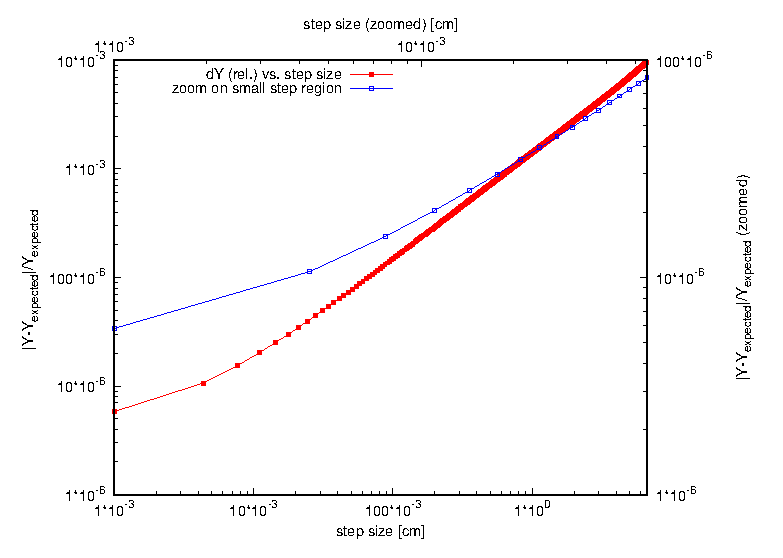
\includegraphics[width=0.5\linewidth]{gnuplot_scanStepSize.eps}

  Obviously, accuracy requires very small step size. This stems from the momentum change
  (integration in magnetic fields allows much greater step size).
\end{minipage}

   \end{document}
